%!TeX TS-program = Lualatex
%!TeX encoding = UTF-8 Unicode
%!TeX spellcheck = en
%!BIB TS-program = biber
% -*- coding: UTF-8; -*-
% vim: set fenc=utf-8
%%%%%%%%%%%%%%%%%%%%%%%%%%%%%%%%%%%%%%%%%%%%%%%%%%%%%%%%%%%%%%%%%%%%%
\documentclass[11pt]{article}
\usepackage[utf8]{inputenc}
\usepackage{times}
\usepackage{wrapfig}
\usepackage{graphicx}
\usepackage{floatrow}
\usepackage{multicol}
\usepackage{amsmath}


\oddsidemargin -0.5in		% margin, in addition to 1" standard
\textwidth 7.5in		% 8.5" - 2*(1+\oddsidemargin)

\topmargin -1in		% in addition to 1.5" standard margin
\textheight 9.75in 		% 11 - ( 1.5 + \topmargin + <bottom-margin> )

\columnsep 0.25in

\parindent 0pt
\parskip 12pt

\flushbottom \sloppy
\pagestyle{empty} % No page numbers

\usepackage{siunitx}%The siunitx package provides a  set  of  tools  for  authors  to  typeset  quantities  in  aconsistent  way.

\newcommand{\ms}{\si{\milli\second}}%

%%%%%%%%%%%%%%%%%%%%%%%%%%%%%%%%%%%%%%%%%%%%%%%%%%%%%%%%%%%%%%%%%%%%%
\usepackage[
%style=chem-acs,
style=numeric,						% numeric style for reference list
citestyle=numeric-comp,
%style=alphabetic-verb,
giveninits=false,
maxbibnames=1,
%firstinits=true,
%style=apa,
%maxcitenames=1,
%maxnames=3,
%minnames=1,
%maxbibnames=99,
dateabbrev=true,
giveninits=true,
%uniquename=init,
url=false,
doi=false,
isbn=false,
eprint=false,
texencoding=utf8,
bibencoding=utf8,
autocite=superscript,
backend=biber,
%sorting=none,
sorting=none,
sortcites=false,
%articletitle=false
]{biblatex}%

\bibliography{ref.bib}
%%%%%%%%%%%%%%%%%%%%%%%%%%%%%%%%%%%%%%%%%%%%%%%%%%%%%%%%%%%%%%%%%%%%%%
\newcommand{\mycaption}[1]{\caption*{#1}}

\usepackage{titlesec}
% \titlespacing*{<command>}{<left>}{<before-sep>}{<after-sep>}
\titlespacing*{\section}
{0pt}{1.5ex}{0.8ex}
\titlespacing*{\subsection}
{0pt}{0.9ex}{0.4ex}
\titlespacing*{\subsubsection}
{0pt}{0.5ex}{0.3ex}
\titlespacing*{\paragraph}{%
  0pt}{%              left margin
  0.0\baselineskip}{% space before (vertical)
  1em}%               space after (horizontal)

\usepackage{setspace}

\begin{document}

%%%-----------------------------------------------------------------
{\Large\bf 
Automatic detection of spiking motifs in multi-unit raster plots
}

%{\bf
%Anonymous submission for double-blind review. \\
%}
\hrule
%%SUMMARY
%%%-----------------------------------------------------------------
\textbf{Summary} %}
Recently, there has been growing interest in the detection of repeating spike patterns in multi-unit raster plots. In this study, we introduce an extension of such detection models by providing a generative model for raster plot synthesis. An optimal detection procedure is derived from this model. This takes the form of a logistic regression coupled with a temporal convolution. We evaluate the ability of this model to detect spike patterns in synthetic data. Since this model is differentiable, we derive an unsupervised learning method in the form of gradient descent on the loss function of an auto-encoder model for the raster using the spike patterns. This unsupervised learning method is able to recover the synthetically generated spike patterns, and we plan to apply it to neurobiological data as well.
\vspace{.5cm}
\hrule
%---------------------------
\textbf{Additional Details.}%


Current technological advances allow simultaneous recording of large numbers of neurons, driving the development of efficient methods for detecting structured patterns in raster plots~\parencite{russo_cell_2017, stella_3d-spade_2019}. Here, we attempt to extend these methods by explicitly representing spike motifs as a temporal pattern of activation of different units. In this way, we can parameterize each motif by the set of tuples that define the weight and delay of each element of the motif. 

%
\begin{figure}[h!]%wrapfigure}{}{\textwidth}
  % \subfloat[M]{%ulti-unit raster]{
    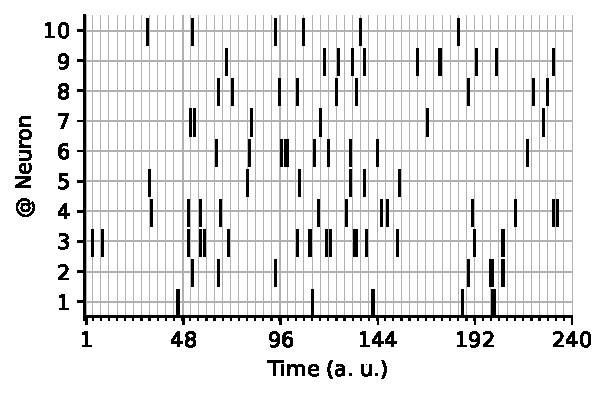
\includegraphics[width=.25\linewidth]{figure_1a_k.pdf}
  % }%
  % %\hfill
  % \subfloat[M]{%Spiking motifs]{
    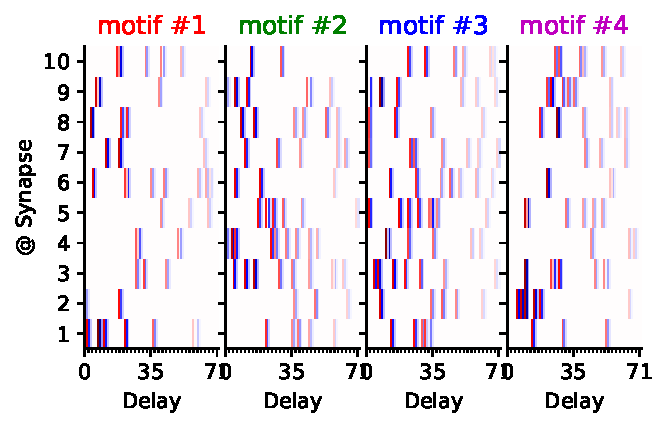
\includegraphics[width=.23\linewidth]{figure_1b.pdf}
  % }%
  % \subfloat[M]{%Raster of motifs]{
  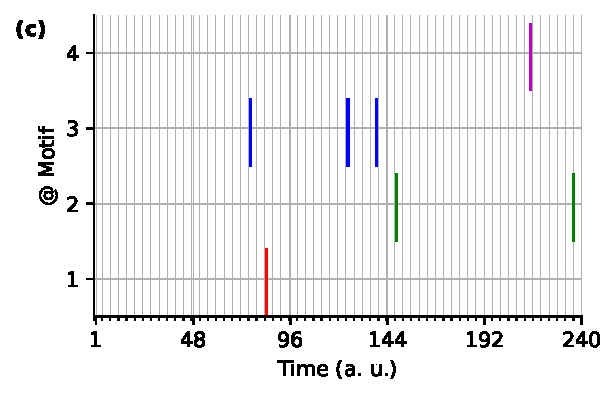
\includegraphics[width=.25\linewidth]{figure_1c.pdf}
  % }%
  % %\hfill
  % \subfloat[M]{%Annotated raster]{
    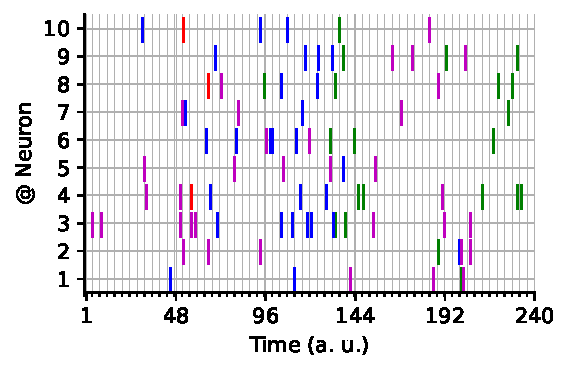
\includegraphics[width=.25\linewidth]{figure_1a.pdf}
  % }
  %\vspace{-55pt}
{
\caption{A multiunit raster plot synthesized from $4$ different spiking motifs. We show these different motifs, each identified at the top by a different color, and each of $10$ neurons from the multi-unit recording and $71$ different possible delays is assigned the evidence of activation (red) or deactivation (blue). The activation in time of the different motifs is then used to define a generative model for drawing a raster plot on the multi-unit address space. By inverting this model, an inference model can be defined for their efficient detection. The original raster plot can be annotated with each identified spiking motif.
}
\label{fig:1}
}
\vspace{-5pt}
\end{figure}%wrapfigure}
%---------------------------
%
% * Limit : not online - in the future it is a model of a neuron
%

By discretizing time (here with an arbitrary time unit $1~\ms$), we can also define the motifs as a matrix giving the weight with respect to the different delays $d \in [0, D]$ (where $D$ is the maximum delay) at different addresses $a \in [1, N]$ where $N$ is the number of neurons from the multiunit recording. 
When a given motif is activated, it will produce a discharge pattern corresponding to that specific set of delays and addresses. 
Let's define the probability of firing of a neuron $a$ at a given time $t$ as a Bernoulli trial whose (only) parameter is a bias $p(t, a) \in [0, 1]$. For any given probability $p$ it is convenient to define the corresponding \emph{evidence} which corresponds to the log odds $\log \frac{p}{1-p} = \sigma^{-1}(p)$, where $\sigma$ is the sigmoid function. 
Assuming that the presence of spiking motifs is binary, it is easy to show that the total evidence can be written as the sum of these evidences, whose values are given by the corresponding weights.
Assuming that we know that there are $M$ such motifs, we define $b \in [1, M]$ the address of a motif and $W_b$ the corresponding weight matrices. This allows us to derive a generative model for raster plots (see figure~\ref{fig:1}).
 Spiking motifs may be activated independently at random times and we write that $B(b, t)=1$ if $b$ is activated at $t$ (and otherwise $B(b, t)=0$). We can thus write the probability bias as %the joint probability given these factors as 
$%$
p(t, a) = \sigma\big(W_0 + \sum_{b, t} B(b, t) \cdot W_b(a, t-d) \big)  
$. We will further assume that the weights are balanced (their mean is zero) and that $W_0$ is a bias such that $p_0=\sigma(W_0)$ is the average background firing rate. Conveniently, this summation can be written as a one-dimensional temporal convolution operator, so we can simply write $p = \sigma(W_0 + B \ast W )$ where  $p\in [ 0, 1]^{N\times T}$ and $B\in \{0, 1\}^{M\times T}$ is the raster plot corresponding to the temporal activation of the spiking motifs. Finally, we obtain the raster plot $A\in \{0, 1\}^{N\times T}$ by drawing spikes using independent Bernoulli trials $A \sim \mathcal{B}(p)$. Note that, depending on the shape of the kernels, the generative model can model a Poisson process, generate rhythmic activity or more generally propagating waves. This formulation thus defines a simple generative model for raster plots as a combination of independent spiking motifs. 

\vspace{25pt}

%---------------------------
\begin{wrapfigure}{r}{.350\textwidth}
% \vspace{-15pt}
%
% ❯ git add figure_N_PG_time.pdf figure_N_PGs.pdf figure_N_pre.pdf
%\subfloat[]{
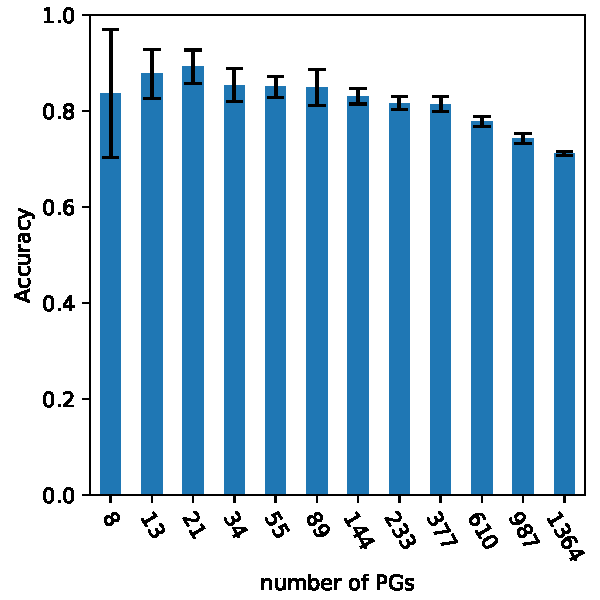
\includegraphics[width=\linewidth]{figure_N_PGs.pdf}
%}%
%\subfloat[]{\includegraphics[width=.49\linewidth]{Figures/fig_methods_nat.pdf}}%
\vspace{-25pt}
{
\caption{Accuracy of detection as a function of the number $M$ of superposed motifs.
}
\label{fig:2}
}
% \vspace{-10pt}
\end{wrapfigure}
%---------------------------
This generative model allows to derive an inference model for the estimation of sources $B$ when observing a raster plot $A$. 
In our specific case, the difference with~\parencite{russo_cell_2017, stella_3d-spade_2019} is that the regression is performed in both dendritic and delay space by extending the summation with a temporal convolution operator. Using this forward model, it is possible to estimate the logit (inverse of a sigmoid) $\hat{B}(b, t)$ for the presence of a motif at address $b$ and time $t$ by using the transpose convolution operator. Thus, when observing $A$, one can infer $\hat{B} = A \ast W^T$ and select the most activated elements. In particular, if we consider weights $W_b$ with similar decreasing exponential time profiles, we can prove that this is similar to finding the tuning function of L-NL neurons, as used in the method of~\parencite{berens_fast_2012}.
Assuming that we know the spiking motifs as defined by the $W_b$ matrices, we quantified the accuracy of detecting the occurrence of spiking motifs as the average number of times that the exact address and time were inferred.  
To quantify the efficiency of this operation, we generated $M=55$ synthetic spiking motifs as random independent kernels over $128$ presynaptic inputs and $D=71$ possible delays. We drew random independent instances of $B$ with a length of $T=1000$ time steps and with an average of $2.0$ occurrences each. This allowed us to generate raster plots which we used to infer $\hat{B}$. We compute the accuracy as the rate of true positive detections and observe on average $\about 98\%$ correct spiking motifs for both address and timing.

%---------------------------
\begin{wrapfigure}{r}{.350\textwidth}
\vspace{-10pt}
% ❯ git add figure_N_PG_time.pdf figure_N_PGs.pdf figure_N_pre.pdf
%\subfloat[]{
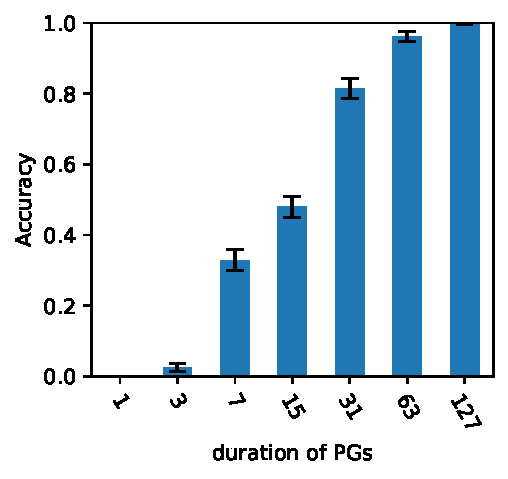
\includegraphics[width=\linewidth]{figure_N_PG_time.pdf}
%}%
%\subfloat[]{\includegraphics[width=.49\linewidth]{Figures/fig_methods_nat.pdf}}%
\vspace{-25pt}
{
\caption{Accuracy of detection as a function of the temporal depth $D$ of motifs.
}
\label{fig:3}
}
% \vspace{-15pt}
\end{wrapfigure}
%---------------------------
We extended this result by showing how accuracy would evolve as a function of the number of simultaneous spiking motifs, while keeping the frequency of occurrence the same. We show in Figure~\ref{fig:2} that the accuracy of finding the right motif is still above $80\%$ accuracy with more than $1364$ spiking motifs. Moreover, we show in Figure~\ref{fig:3} that (with $M=55$ spiking motifs fixed) the accuracy increases sharply as the temporal depth $D$ of the spiking motifs is increased. This quantitatively demonstrates the potential of using codes with spiking motifs. 

These results were obtained while assuming that we know $W$. However, this is in general not the case, for instance when observing the raster plot of a population of neurons. Inspired by the k-means algorithm, it is possible to devise a self-supervised learning algorithm for the automatic detection of spiking motifs. 

% learning
The underlying metric is the binary cross-entropy, as used in the logistic regression model.

Our preliminary results show that it is possible to retrieve spiking motifs embedded in the data, yet that further analysis is necessary to improve the convergence of the algorithm. In particular, it seems promising to use a sparseness constraint in the inference mechanism such as to remove spurious correlations in the inference.
%
\printbibliography
\end{document}
